\clearpage % clear the prior chapter's page

\chapter{Alternating access in LeuT-fold transporters}\label{ch:leutintro}
%\vspace{-7mm}
%\bigskip

\section{Introduction}
Secondary active transporters tap the potential energy stored in electrochemical gradients to allow cells to import and export nutrients and cytotoxic drugs as needed \citep*{Bosshart2019}. Despite a divergence in topologies and ligands \citep*{Drew2016, Shi2013}, these transporters are believed to operate via alternating access, a generic term referring to the exposure of the substrate-binding site to no more than one side of the membrane at a time \citep*{Jardetzky1966, Mitchell1957}. This mechanism allows transporters to couple conformational changes critical to substrate binding and/or release while minimizing the uncoupled flux or leaking of ions down their electrochemical gradients. Although this basic working model of transport has been devised over sixty years ago \citep*{Jardetzky1966}, characterizing the precise molecular mechanisms relating substrate binding to translocation in individual proteins of interest presents a formidable scientific challenge. High-resolution structures cannot identify the movements underpinning alternating access unless a protein is captured in multiple distinct conformations \citep*{Hofmann2019, Perez2012}. As such, solution-state measurements, carried out in the absence or presence of various substrates under conditions permitting conformational interconversion, directly report on the transporter's energy landscapes and allows high-resolution snapshots to be assigned to specific intermediate states observed in the functional cycle \citep*{Juette2014, Liapakis1999, Mchaourab2011, Oganesyan2018}. Unfortunately, but not unexpectedly, few proteins have been so exhaustively characterized.

\begin{figure}[h!]
\centering
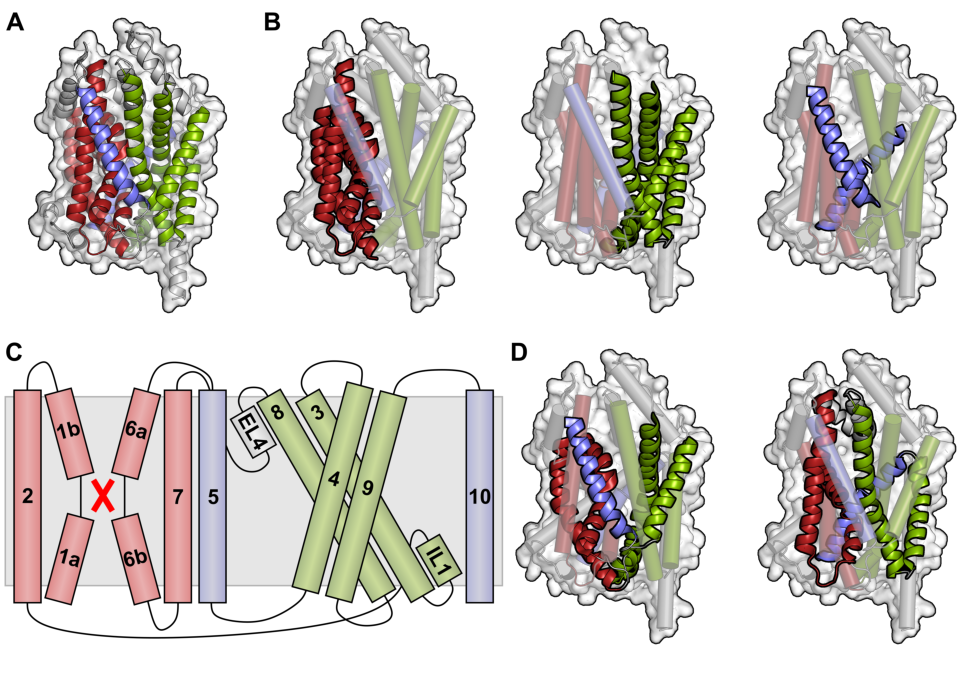
\includegraphics[width=6.5in]{Figures/leutintro_arch.pdf}
 \caption[Architecture of the bacterial amino acid transporter LeuT.]{Architecture of the bacterial amino acid transporter LeuT. (A) The sodium-coupled amino acid transporter LeuT. (B) The ten-transmembrane helix core consists of a bundle domain (highlighted in red), a hash domain (green), and a pair of gating helices (blue). (C) Cartoon depiction of the conserved transport domain showing the pseudo-twofold symmetry of the ten-helix core. Substrate-binding site indicated by the red X. (D) Inverted repeats in helices 1-5 and 6-10.}
\label{fig:leutintro_arch}
\end{figure}

The bacterial \gls{nss} homolog LeuT found in the thermophilic archaea \emph{Aquifex aeolicus} presents a rare example of a transporter that has been studied to this extent (Figure \ref{fig:leutintro_arch}) \citep*{Yamashita2005}. LeuT couples the import of small aliphatic amino acids such as leucine and alanine to an inward sodium gradient and an outward proton gradient \citep*{Zhao2010}. Nearly two decades of persistent investigation has produced a library of atomic-resolution crystal structures capturing conformational intermediate states \citep*{Fan2021, Gotfryd2020, Krishnamurthy2012, Malinauskaite2016, Singh2008, Yamashita2005} linked by solution-state experimental data collected using various techniques \citep*{Adhikary2017, Billesbølle2015, Billesbølle2016, Claxton2010, Kazmier2014a, Merkle2018, Zhao2011}. Collectively, this body of knowledge describes in exquisite detail the molecular and energetic basis of ligand-dependent conformational changes driving sodium-coupled amino acid transport.

In this chapter, we explore the extent to which structural homologs of LeuT, many of which are found in humans and whose dysfunction contribute to a range of diseases, undergo similar ligand-dependent structural rearrangements \citep*{Loland2015}. These homologs include mammalian \gls{nss}s, such as \gls{sert} and \gls{dat} \citep*{Beuming2006, Coleman2016, Penmatsa2013}, as well as a multitude of more distant homologs that have been identified across nearly a dozen families (Tables \ref{tab:leutintro_proteins1} and \ref{tab:leutintro_proteins2}). As many proteins with the LeuT-fold have been the subject of extensive study over the course of many decades and have been the subject of numerous recent reviews \citep*{Bozzi2021, Cheng2019, Chew2021,  ErrastiMurugarren2021, Henriquez2021, Krammer2019, Patching2018, Rudnick2019, Singh2018, Ziegler2010}, this chapter focuses on comparing their conformational changes, structural dynamics, and energy landscapes. Necessarily, emphasis is placed on \gls{nss}s which are the most extensively studied family of transporters with this topology.

\begin{table}[h!]
\scriptsize
\renewcommand{\tabcolsep}{0.09cm}
\centering
\caption[Curated library of LeuT-fold protein structures.]{Curated library of LeuT-fold protein structures. Conformations are assigned to either \gls{ofop}, \gls{ofoc}, \gls{oo}, \gls{ifoc}, or \gls{ifop}. Structures are marked if they were mutated ($\dagger$) or bound to inhibitors ($\ddagger$) or antibodies ($\mathsection$). Redundant structures have been omitted.}

%\newcolumntype{Y}{>{\raggedright\arraybackslash}X}

% Structures are marked if they were mutated ($\dagger$) or bound to inhibitors ($\ddagger$) or antibodies ($\mathsection$).}

\begin{center}
\begin{tabular}{l l l l l r}
\toprule \\
\textbf{Protein \emph{(Organism)}} & \textbf{Conf.} & \textbf{PDB ID} & \textbf{Resolution} & \textbf{Substrates} & \textbf{Reference} \\
\midrule \\

\multicolumn{5}{l}{\textbf{Neurotransmitter-sodium symporter family}} \\
$\mathrm{b^{0}AT1}$ \emph{(Homo sapiens)} & \gls{ofoc} & 6M17 & 2.90 \AA & Apo & \citep*{Yan2020b} \\
DAT \emph{(Drosophila melanogaster)} & \gls{ofop} & $\mathrm{4XP1^\mathsection}$ & 2.89 \AA & $\mathrm{2Na^+/Cl^-/Dopamine}$ & \citep*{Penmatsa2015} \\
GlyT1 \emph{(Homo sapiens)} & \gls{ifop} & $\mathrm{6ZPL}^{\dagger \ddagger \mathsection}$ & 3.94 \AA & $ \mathrm{2Na^+/Cl^-/Benzoylisoindoline}$ & \citep*{Shahsavar2021} \\
LeuT \emph{(Aquifex aeolicus)} & \gls{ofop} & $\mathrm{3TT1^{\dagger \mathsection}}$ & 3.10 \AA & $\mathrm{2Na^+}$ & \citep*{Krishnamurthy2012} \\
& & $\mathrm{3F3A^{\ddagger}}$ & 2.00 \AA & $\mathrm{2Na^+/Tryptophan}$ & \citep*{Singh2008} \\
& & 7DIXb & 3.49 \AA & $\mathrm{Na^+/Leucine}$ & \citep*{Fan2021} \\
& \gls{ofoc} & 2A65 & 1.65 \AA & $\mathrm{2Na^+/Leucine}$ & \citep*{Yamashita2005} \\
& & 5JAE & 2.50 \AA & Apo & \citep*{Malinauskaite2016} \\
& \gls{ifoc} & $\mathrm{6XWM^\dagger}$ & 2.60 \AA & $\mathrm{2Na^+/Phenylalanine}$ & \cite*{Gotfryd2020} \\
& \gls{ifop} & $\mathrm{3TT3^{\dagger \mathsection}}$ & 3.22 \AA & Apo & \citep*{Krishnamurthy2012} \\
MhsT \emph{(Bacillus halodurans)} & \gls{ifoc} & 4US3 & 2.10 \AA & $\mathrm{2Na^+/Tryptophan}$ & \citep*{Malinauskaite2014} \\
SERT \emph{(Homo sapiens)} & OFOp & $\mathrm{5I6Z^{\dagger \mathsection}}$ & 4.53 \AA & Apo & \citep*{Coleman2016} \\
& & $\mathrm{5I6X^{\dagger \ddagger \mathsection}}$ & 3.14 \AA & Paroxetine & \citep*{Coleman2016} \\
& \gls{ifoc} & $\mathrm{6DZZ^{\ddagger \mathsection}}$ & 3.60 \AA & Ibogaine & \citep*{Coleman2019} \\
\\
\multicolumn{5}{l}{\textbf{Amino acid-polyamine-organocation transporter family}}
\\
AdiC \emph{(Escherichia coli)} & OFOp & 3OB6 & 3.00 \AA & Arginine & \citep*{Kowalczyk2011} \\
& & 5J4I & 2.21 \AA & Apo & \citep*{Ilgu2016} \\
& & 5J4N & 2.59 \AA & Agmatine & \citep*{Ilgu2016} \\
& \gls{ofoc} & $\mathrm{3L1L^{\dagger}}$ & 3.00 \AA & Arginine & \citep*{Fang2009} \\
AdiC \emph{(Salmonella typhimurium)} & \gls{ofop} & 3NCY & 3.20 \AA & Apo & \citep*{Fang2009} \\
ApcT \emph{(Methanococcus janaschii)} & \gls{ifoc} & 3GIA & 2.32 \AA & Apo & \citep*{Shaffer2009} \\
$\mathrm{b^{(0,+)}AT1}$ \emph{(Homo sapiens)} & \gls{ifop} & 6LI9 & 2.30 \AA & Arginine & \citep*{Yan2020a} \\ 
& & 6LID & 2.70 \AA & Apo & \citep*{Yan2020a} \\
BasC \emph{(Carnobacterium} sp. AT7\emph{)} & \gls{ifop} & $\mathrm{6F2W^{\mathsection}}$ & 3.40 \AA & 2-Aminoisobutyrate & \citep*{Errasti-Murugarren2019} \\
& & $\mathrm{6F2G^{\mathsection}}$ & 2.92 \AA & Apo & \citep*{Errasti-Murugarren2019} \\
GadC \emph{(Escherichia coli)} & \gls{ifop} & 4DJI & 3.19 \AA & Apo & \citep*{Ma2012} \\
GkApcT \emph{(Geobacillus kaustophilus)} & \gls{ifoc} & 5OQT & 2.86 \AA & Alanine & \citep*{Jungnickel2018} \\
& & 6F34 & 3.13 \AA & Arginine & \citep*{Jungnickel2018} \\
Lat1 \emph{(Homo sapiens)} & \gls{ofop} & $\mathrm{7DSQ^{\ddagger}}$ & 3.40 \AA & Diiodotyrosine & \citep*{Yan2021} \\
& \gls{ifop} & $\mathrm{6IRS^{\ddagger}}$ & 3.30 \AA & JPH203 & \citep*{Yan2019} \\
& & $\mathrm{6IRT^{\ddagger}}$ & 3.50 \AA & BCH & \citep*{Yan2019} \\
& & $\mathrm{6JMQ^{\mathsection}}$ & 3.31 \AA & Apo & \citep*{Lee2019} \\
Lat2 \emph{(Homo sapiens)} & \gls{ifop} & 7CMH & 3.40 \AA & Tryptophan & \citep*{Yan2020} \\
xCT \emph{(Homo sapiens)} & \gls{ifop} & $\mathrm{7CCS^{\dagger}}$ & 6.20 \AA & Apo & \citep*{Oda2020} \\
\\
\multicolumn{5}{l}{\textbf{Cation-chloride cotransporter family}} \\
NKCC1 \emph{(Homo sapiens)} & \gls{ifop} & 6PZT & 3.46 \AA & Apo & \citep*{Yang2020} \\
NKCC1 \emph{(Danio rerio)} & \gls{ifop} & 6NPL & 2.90 \AA & $\mathrm{K^+/2Cl^-}$ & \citep*{Chew2019} \\
KCC1 \emph{(Homo sapiens)} & \gls{ifop} & 6KKT & 2.90 \AA & $\mathrm{K^+/2Cl^-}$ & \citep*{Liu2019} \\
& & 6KKR & 2.90 \AA &  Apo & \citep*{Liu2019} \\
KCC2 \emph{(Homo sapiens)} & \gls{ifop} & 7D8Z & 3.40 \AA & Apo & \citep*{Xie2020} \\
KCC3 \emph{(Homo sapiens)} & \gls{ifop} & $\mathrm{6M22^{\ddagger}}$ & 2.70 \AA & DIOA & \citep*{Chi2021} \\
& & 7D90 & 3.60 \AA & Apo & \citep*{Xie2020} \\
KCC4 \emph{(Homo sapiens)} & \gls{ifop} & 7D99 & 2.90 \AA & Apo & \citep*{Xie2020} \\
KCC4 \emph{(Mus musculus)} & \gls{ifop} & 6UKN & 3.65 \AA & $\mathrm{K^+/Cl^-}$ & \citep*{Reid2020} \\
\bottomrule \\
\end{tabular} 
\end{center}
\label{tab:leutintro_proteins1}
\end{table}

\begin{table}[h!]
\scriptsize
\renewcommand{\tabcolsep}{0.15cm}
\centering
\caption[Curated library of LeuT-fold protein structures (continued).]{Curated library of LeuT-fold protein structures (continued).}

%\newcolumntype{Y}{>{\raggedright\arraybackslash}X}

% Structures are marked if they were mutated ($\dagger$) or bound to inhibitors ($\ddagger$) or antibodies ($\mathsection$).}

\begin{center}
\begin{tabular}{l l l l l r}
\toprule \\
\textbf{Protein \emph{(Organism)}} & \textbf{Conf.} & \textbf{PDB ID} & \textbf{Resolution} & \textbf{Substrates} & \textbf{Reference} \\
\midrule \\
\multicolumn{5}{l}{\textbf{Betaine/carnitine/choline transporter family}} \\
BetP \emph{(Corynebacterium glutamicum)} & \gls{ofop} & $\mathrm{4DOJb^{\dagger}}$ & 3.25 \AA &Apo & \citep*{Perez2012} \\
& \gls{ofoc} & $\mathrm{4DOJa^{\dagger}}$ & 3.25 \AA & Apo & \citep*{Perez2012} \\
& \gls{oo} & 4AINa & 3.10 \AA & Apo & \citep*{Perez2012} \\
& \gls{ifoc} & 2WIT & 3.35 \AA & $\mathrm{2Na^+/Betaine}$ & \citep*{Ressl2009} \\
& \gls{ifop} & 3P03 & 3.35 \AA & $\mathrm{2Na^+/Choline}$ & \citep*{Perez2011} \\
CaiT \emph{(Escherichia coli)} & \gls{ifop} & 2WSX & 3.50 \AA & $\mathrm{\upgamma}$-Butyrobetaine & \citep*{Schulze2010} \\
& & 3HFX & 3.15 \AA & Carnitine & \citep*{Tang2010} \\
CaiT \emph{(Proteus mirabilis)} & \gls{ifop} & 2WSW & 2.29 \AA & Apo & \citep*{Schulze2010} \\
\\
\multicolumn{5}{l}{\textbf{Natural resistance-associated macrophage protein family}} \\
ScaDMT \emph{(Staphylococcus capitis)} & \gls{ifop} & $\mathrm{5M94^{\dagger \mathsection}}$ & 3.10 \AA & Apo & \citep*{Ehrnstorfer2014} \\ 
& & $\mathrm{5M95^{\dagger \mathsection}}$ & 3.40 \AA & $\mathrm{Mn^{2+}}$ & \citep*{Ehrnstorfer2014} \\ 
EcoDMT \emph{(Eremococcus coleocola)} & \gls{ofop} & $\mathrm{5M8K}^{\dagger}$ & 3.60 \AA & Apo & \citep*{Ehrnstorfer2017} \\
& & $\mathrm{5M87}^{\dagger}$ & 3.30 \AA & $\mathrm{Mn^{2+}}$ & \citep*{Ehrnstorfer2017} \\
DraNramp \emph{(Deinococcus radiodurans)} & \gls{ofop} & $\mathrm{6D91^{\dagger}}$ & 2.36 \AA & Apo & \citep*{Bozzi2019} \\
& & $\mathrm{6BU5^{\dagger}}$ & 3.30 \AA & $\mathrm{Mn^{2+}}$ & \citep*{Bozzi2019} \\
& \gls{ifoc} & $\mathrm{6C3I^{\dagger}}$ & 2.40 \AA & Apo & \citep*{Bozzi2019} \\
& \gls{ifop} & $\mathrm{5KTE^{\dagger \mathsection}}$ & 3.94 \AA & Apo & \citep*{Bozzi2016} \\
& & $\mathrm{6D9W^{\dagger \mathsection}}$ & 3.94 \AA & Apo & \citep*{Bozzi2019} \\
\\
\multicolumn{5}{l}{\textbf{Sodium-solute symporter family}} \\
vSGLT \emph{(Vibrio parahaemolyticus)} & \gls{ifoc} & 3DH4 & 2.70 \AA & $\mathrm{2Na^+/Galactose}$ & \citep*{Faham2008} \\
& \gls{ifop} & $\mathrm{2XQ2^{\dagger}}$ & 2.70 \AA & Apo & \citep*{Watanabe2010} \\
SiaT \emph{(Proteus mirabilis)} & \gls{ofop} & 5NV9 & 1.95 \AA & $\mathrm{2Na^+/}$Neuraminic acid & \citep*{Wahlgren2018} \\
& & 5NVA & 2.26 \AA & Apo &  \citep*{Wahlgren2018} \\
\\
\multicolumn{5}{l}{\textbf{Potassium uptake permease family}} \\
KimA \emph{(Bacillus subtilis)} & \gls{ifop} & 6S3K & 3.70 \AA & $\mathrm{3K^+}$ & \citep*{Tascon2020} \\
\\
\multicolumn{5}{l}{\textbf{Amino acid-auxin permease family}} \\
DrSLC38A9 \emph{(Danio rerio)} & \gls{ifop} & $\mathrm{6C08^{\dagger \mathsection}}$ & 3.17 \AA & Arginine & \citep*{Lei2018} \\
& & $\mathrm{7KGV^{\dagger \mathsection}}$ & 3.40 \AA & Apo & \citep*{Lei2021} \\
\\
\multicolumn{5}{l}{\textbf{Nucleobase-cation symporter-1 family}} \\
Mhp1 \emph{(Microbacterium tumefaciens)} & \gls{ofop} & 2JLN & 2.85 \AA & Apo & \citep*{Weyand2008} \\
& \gls{ofoc} & 4D1B & 3.80 \AA & $\mathrm{Na^+/Benzylhydantoin}$ & \citep*{Simmons2014} \\
& \gls{ifop} & 2X79 & 3.80 \AA & Apo & \citep*{Shimamura2010} \\
\\
\multicolumn{5}{l}{\textbf{Alanine/glycine-cation symporter family}} \\
AgcS \emph{(Methanococcus maripaludis)} & \gls{oo} & $\mathrm{6CSE^{\mathsection}}$ & 3.24 \AA & $\mathrm{Na^+/Alanine}$ & \citep*{Ma2018} \\
& & $\mathrm{6CSF^{\mathsection}}$ & 3.30 \AA & $\mathrm{Na^+/}$D-Alanine & \citep*{Ma2018} \\
\bottomrule \\
\end{tabular} 
\end{center}
\label{tab:leutintro_proteins2}
\end{table}

\section{Functional and structural diversity within the fold}

\subsection{The ten transmembrane helix topology}

Proteins in the LeuT-fold belong to the \gls{apc} superfamily of transporters \citep*{Vastermark2014} and share a core transport structure consisting of ten \gls{tmh}s related by pseudo-twofold symmetry \citep*{Forrest2008, Kazmier2017}. These ten helices can be subdivided into three domains: the bundle domain (\gls{tmh} 1, 2, 6, and 7), the hash domain (\gls{tmh} 3, 4, 8, and 9), and gating helices (\gls{tmh} 5 and 10; this Chapter uses this canonical numbering scheme and ignores N-terminal transmembrane helices). Additional N- and/or C-terminal helices uninvolved in transport flank this ten-helix core and vary across individual transporter families comprising the LeuT fold. Characteristically, \gls{tmh} 1 and 6 contain conserved unwound regions, observed near the geometric center of the ten-helix core, and their involvement in ligand coordination is a hallmark of the fold \citep*{Screpanti2007}. Importantly, structural similarity is not accompanied by sequence similarity: few structural motifs are identifiable at the sequence level \citep*{Billesbølle2015, Malinauskaite2014, Stolzenberg2017}, which prevented these protein families from being co-categorized prior to the determination of their structures \citep*{Beuming2006}.

\begin{figure}[h!]
\centering
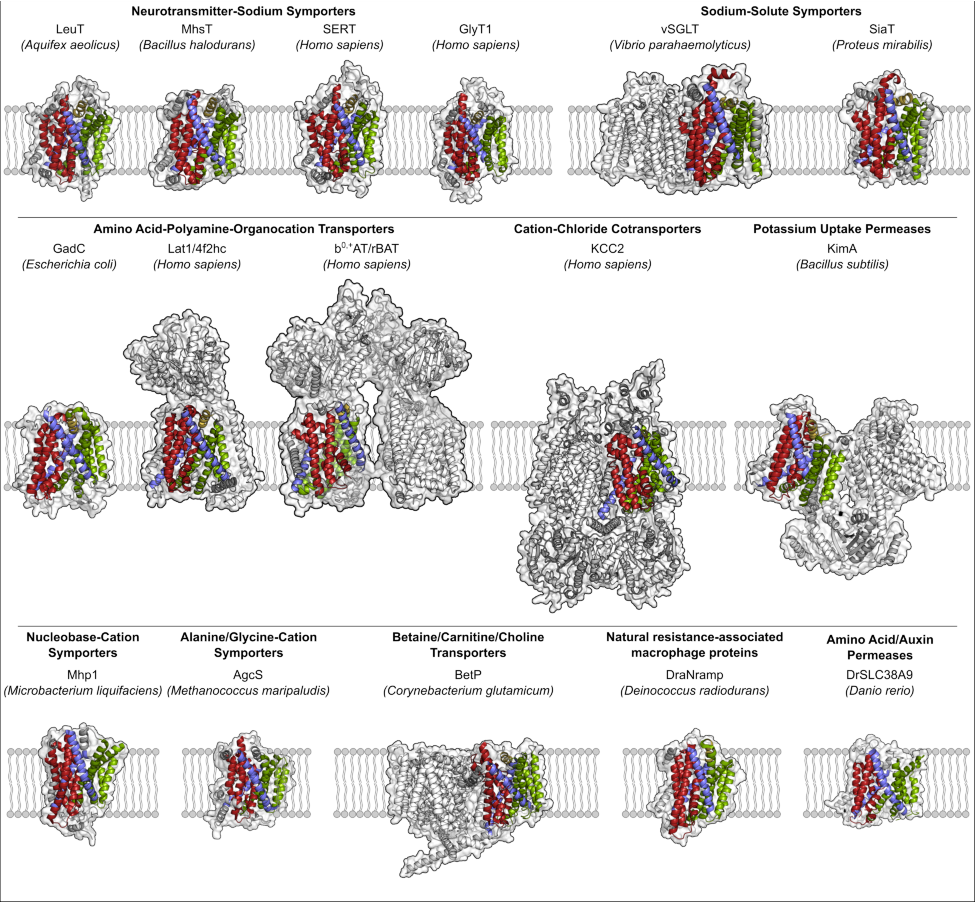
\includegraphics[width=6.5in]{Figures/leutintro_panel.pdf}
 \caption[Structural diversity within the LeuT fold.]{Structural diversity within the LeuT fold. The LeuT fold is adopted by proteins found in a range of transporter families. PDB IDs, starting from top left: 2A65, 4US4, 5I6X, 6PZL, 3DH4, 5NVA; 4DJI, 6IRS, 6LI9, 6M23, 6S3K; 2JLN, 6CSE, 2WIT, 6D91, 6C08.}
\label{fig:leutintro_panel}
\end{figure}

The LeuT fold is perhaps best defined by its evolutionary persistence across families of transporters with sequences that appear unrelated (Figure \ref{fig:leutintro_panel}) \citep*{Abramson2009}. In addition to \gls{nss} \citep*{Cheng2019}, the LeuT fold has been found to be adopted by members of the \gls{sss} \citep*{Henriquez2021}, \gls{ccc} \citep*{Chew2021}, \gls{apc} transporter \citep*{ErrastiMurugarren2021}, \gls{nramp} \citep*{Bozzi2021}, \gls{ncs} \citep*{Patching2018}, and \gls{aaap} families. The same topology also describes representatives of proteins families unique to prokaryotes, such as those in the \gls{bcct} \citep*{Ziegler2010}, \gls{agcs}, and \gls{kup} families. Additionally, several transporter families lacking representatives in the PDB are predicted to have this fold (Figure \ref{fig:leutintro_unknowns}) \citep*{Saier2016, Tunyasuvunakool2021, Vastermark2014}.

\begin{figure}[h!]
\centering
\includegraphics[width=5.5in]{Figures/leutintro_unknowns.pdf}
 \caption[Predicted structural models of proteins belonging to LeuT-fold families with no representatives in the PDB.]{Predicted structural models of proteins belonging to LeuT-fold families with no representatives in the PDB. Transporter families are defined by the Transporter Classification Database, and each model was generated using AlphaFold2.}
\label{fig:leutintro_unknowns}
\end{figure}

\subsection{Functional variation within the LeuT fold}

Retention of this ten-helix core is all the more remarkable considering the extent to which the functions, ligands, and sequences of these proteins differ. Although the majority of LeuT-fold proteins studied thus far cotransport their substrates and driving ions, others exchange them in opposite directions (symport and antiport, respectively \citep*{Forrest2009}). The centrally located substrate-binding site, shared by symporters and antiporters, accommodates ligands ranging in size and charge from halogen ions and divalent metals to sugars and aromatic amino acids. Its manipulation by mutagenesis has been shown to alter substrate specificity profiles in LeuT (\gls{nss}) \citep*{Piscitelli2011, Zomot2007}, GAT-1 (\gls{nss}) \citep*{Zomot2007}, and BetP (\gls{bcct}) \citep*{Perez2014}, highlighting the involvement of this region in identifying and trafficking ligands.

Beyond plasticity at this specific site, structural features decorating the core transporter further contribute to functional specialization. A remarkable example is SLC38A9, which both exports amino acids from the lysosome and activates the regulatory complex mTORC1 under nutrient-rich conditions \citep*{Rebsamen2015, Wang2015}. An N-terminal domain elegantly couples these two functions by binding to the cytoplasmic cavity \citep*{Lei2021} and, following displacement by the transported substrate arginine, releases and binds to GTPases involved in downstream signaling \citep*{Fromm2020}. In an interesting case of convergent evolution, the C-terminal domain of the pH-dependent \gls{glu}/\gls{gaba} exchanger GadC arrests transport by binding to the intracellular cavity at neutral pH in a nearly identical conformation \citep*{Ma2012}. Autoinhibition by disordered terminal domains has also been directly visualized in several potassium-chloride symporters \citep*{Chi2021, Xie2020}. In other proteins, such as eukaryotic \gls{nss}s, disordered termini instead regulate transport by interacting with a range of cytoplasmic proteins \citep*{Cooper2019, Karam2018}. In BetP, a cytoplasmic C-terminal helical domain regulates transport in response to osmotic stress \citep*{Gueler2016, Kraemer2009}. These domains often go unobserved in structural studies \citep*{Coleman2016, Liu2019, Penmatsa2013} due to truncation or intrinsic disorder, prompting speculation regarding their role in transport.

\newpage

\subsection{Quaternary structures adopted by LeuT-fold transporters}

Recent structures obtained by \gls{cryoem} have bolstered the diversity of quaternary structures known to be adopted by these proteins. Whereas X-ray crystallography demonstrated that LeuT-fold transporters can assemble as homodimers (AdiC, vSGLT) \citep*{Faham2008, Gao2009}, homotrimers (BetP, CaiT) \citep*{Ressl2009, Schulze2010}, or heterodimers (GkApcT) \citep*{Jungnickel2018}, due to technical limitations only compact binding interfaces were observed. By contrast, oligomers visualized by \gls{cryoem} reveal a multitude of weaker, more flexible, and in some cases asymmetric binding interfaces \citep*{Chew2019, Lee2019, Oda2020, Tascon2020, Yan2020a, Yan2020b, Yan2019, Yan2020}. For example, the eukaryotic \gls{apc} transporters Lat1, Lat2, and xCT each associate with 4f2hc (also called CD98hc) \citep*{Jeckelmann2020, Oda2020, Yan2019, Yan2020}, a protein with a large extracellular domain and a single transmembrane helix that is uninvolved in transport (Figure \ref{fig:leutintro_panel}). The homologous \gls{apc} transporter $\mathrm{b^{(0,+)}AT1}$ further assembles into a dimer of dimers with rBAT, each of which resemble the Lat/4f2hc complexes \citep*{Wu2020, Yan2020a}. This dimer-of-dimers arrangement was even observed in the \gls{nss} $\mathrm{b^{0}AT1}$, which associates with Angiotensin-converting enzyme 2 (the experimental structure of this tetramer was determined as part of a larger complex involving the SARS-CoV-2 spike protein) \citep*{Yan2020b}. Notably, the N-terminal transmembrane helices of rBAT and 4f2hc bind to the hash domains of $\mathrm{b^{(0,+)}AT1}$ and the Lats, respectively, at a similar position as the C-terminal transmembrane helix of ACE2 to $\mathrm{b^{0}AT1}$. Separately, the eukaryotic \gls{ccc}s \citep*{ Chew2019, Chi2020, Liu2019, Reid2020, Yang2020} and the bacterial potassium transporter KimA \citep*{Tascon2020} both fold as homodimers with large domain-swapped cytoplasmic regions. Divergence in both the sequences of these protein families and the structures of their cytoplasmic domains may highlight a recurrent quaternary assembly mechanism, the extent of which has not yet come to light.

Finally, in many cases, the oligomeric interfaces observed by \gls{cryoem} appear to be weaker and more flexible than suggested by the crystal structures. In both Lat1 and KCC1, for example, substantial interdomain movements have been reported when comparing their respective inward-facing apo and outward-facing inhibitor-bound states \citep*{Liu2019, Yan2021, Yan2019, Yan2020, Zhao2020}. Molecular dynamics simulations of the homodimer KimA suggested that contacts between the two transport domains are transient and fleeting, as these domains are tethered to one another only by their intertwined cytoplasmic domains \citep*{Tascon2020}; similar observations were experimentally made in \gls{ccc}s \citep*{Chi2021}. Such arrangements sharply contrast with the interfaces observed in vSGLT \citep*{Faham2008, Watanabe2010}, BetP \citep*{Ressl2009}, and other oligomers determined by crystallography, and hint at future discoveries regarding how these transporters interact as part of larger complexes.

\subsection{Recurring elements of substrate binding}\label{sec:ligands}

These unique structural features and arrangements surround a highly conserved ten-helix architecture shown in Figure \ref{fig:leutintro_arch}.C that, in several cases, have been shown to retain ligand-binding modes across distantly related proteins (Figure \ref{fig:leutintro_ligands}). A widely discussed example is the conserved sodium site, termed Na2, found in the majority of sodium-coupled symporters \citep*{Faham2008, Ressl2009, Wahlgren2018, Weyand2008, Yamashita2005}. In fact, the Na2 site's recurrence in this fold prompted Chew \emph{et al.} to assign its position to the sodium-binding site in the sodium/potassium/chloride symporter NKCC1, which was subsequently corroborated by molecular dynamics simulations and mutagenesis experiments that severely abrogated transport \citep*{Chew2019, Janos2021}. Among symporters that bind two sodium ions (\gls{nss}s, SiaT \citep*{Wahlgren2018}, BetP \citep*{Khafizov2012}), no such conservation is observed in the position of the other sodium ion. In proton-coupled symporters and amino acid exchangers, positively-charged residues occupy this position (lysine in ApcT, GkApcT, and BasC, and arginine in CaiT \citep*{Errasti-Murugarren2019, Gao2009, Jungnickel2018, Schulze2010, Tang2010}), highlighting the malleability of substrate coupling throughout the fold. A noteworthy exception is the sodium-coupled amino acid symporter AgcS, which coordinates its only sodium at a position equivalent to LeuT's Na1 site, leaving the Na2 site unoccupied \citep*{Ma2018}. This is despite its alanine binding site overlapping nearly perfectly with the substrate binding sites of unrelated amino acid transporters from the \gls{nss} and \gls{apc} families (Figure \ref{fig:leutintro_ligands}.C). To our knowledge, no cations besides sodium ions and protons have been observed in this site, and no comparable degree of structural conservation has observed at other ligand-binding sites, such as those involved in binding potassium (transported by \gls{sert}, as well as the \gls{kup} and \gls{ccc} families) or chloride (transported by \gls{nss}s and \gls{ccc}s).


\begin{figure}[h]
\centering
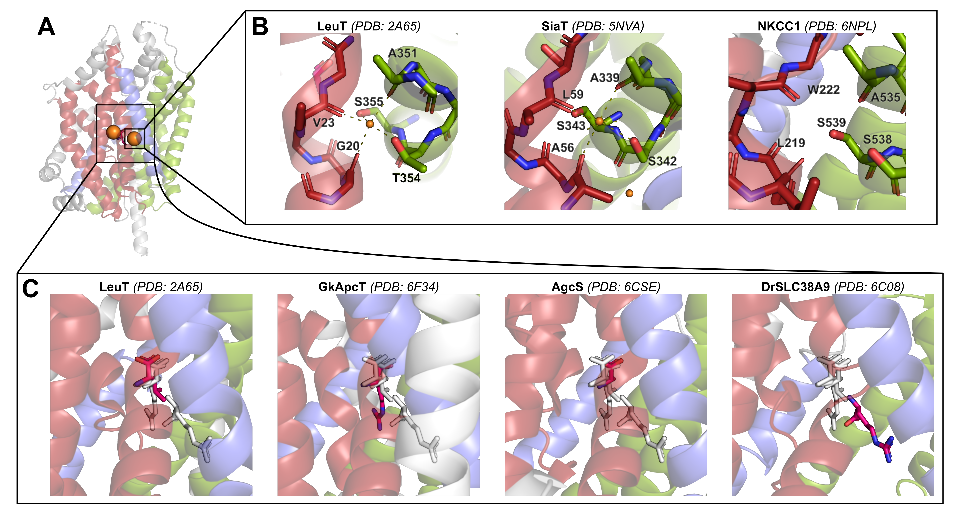
\includegraphics[width=6.5in]{Figures/leutintro_ligands_hoz.pdf}
 \caption[Examples of conserved ligand coordination.]{Examples of conserved ligand coordination. (A) Sodium ions (orange) and leucine (pink) in LeuT. (B) Conservation of the Na2 site. (C) Partial recurrence of amino acid binding modes. Substrates colored white are shared in all four panels.}
\label{fig:leutintro_ligands}
\end{figure}


\section{Alternating access inferred from crystal and cryo-EM structures}

At the molecular level, alternating access involves the opening and closing of gates providing passage to the substrate-binding site from either the intracellular or extracellular spaces \citep*{Jardetzky1966} For transporters with the LeuT-fold, this principally manifests as isomerization between \gls{of} and \gls{if} states using a "rocking bundle" mechanism that forbids substrate entry and exit from the cytoplasmic or periplasmic side of the membrane, respectively \citep*{Forrest2009}. Despite their co-classification, however, closer examination at structural changes in these proteins reveals a striking lack of consensus over the molecular details of alternating access. Conformational divergence as the rule, not the exception, became apparent nearly a decade ago with the publication of high-resolution structures of Mhp1 \citep*{Shimamura2010, Weyand2008}, BetP \citep*{Ressl2009}, and LeuT \citep*{Kazmier2017, Krishnamurthy2012, Yamashita2005}, and has since been reinforced by similar studies in SERT \citep*{Coleman2016, Coleman2019}, DraNramp \citep*{Bozzi2016, Bozzi2019}, and Lat1/4f2hc (Figure \ref{fig:leutintro_aa}) \citep*{Yan2021, Lee2019, Yan2021}. Additional structures of AdiC \citep*{Fang2009, Gao2009} and vSGLT \citep*{Faham2008, Watanabe2010} in both open and occluded conformations, though limited to \gls{of} and \gls{if} states, respectively, further expand the ways in which these transporters grant access to the substrate-binding site. Overall, comparison of pairs of structures reveals fundamental differences in which helices move and which stay fixed (Figure \ref{fig:leutintro_rmsf}).

\begin{figure}[h!]
\centering
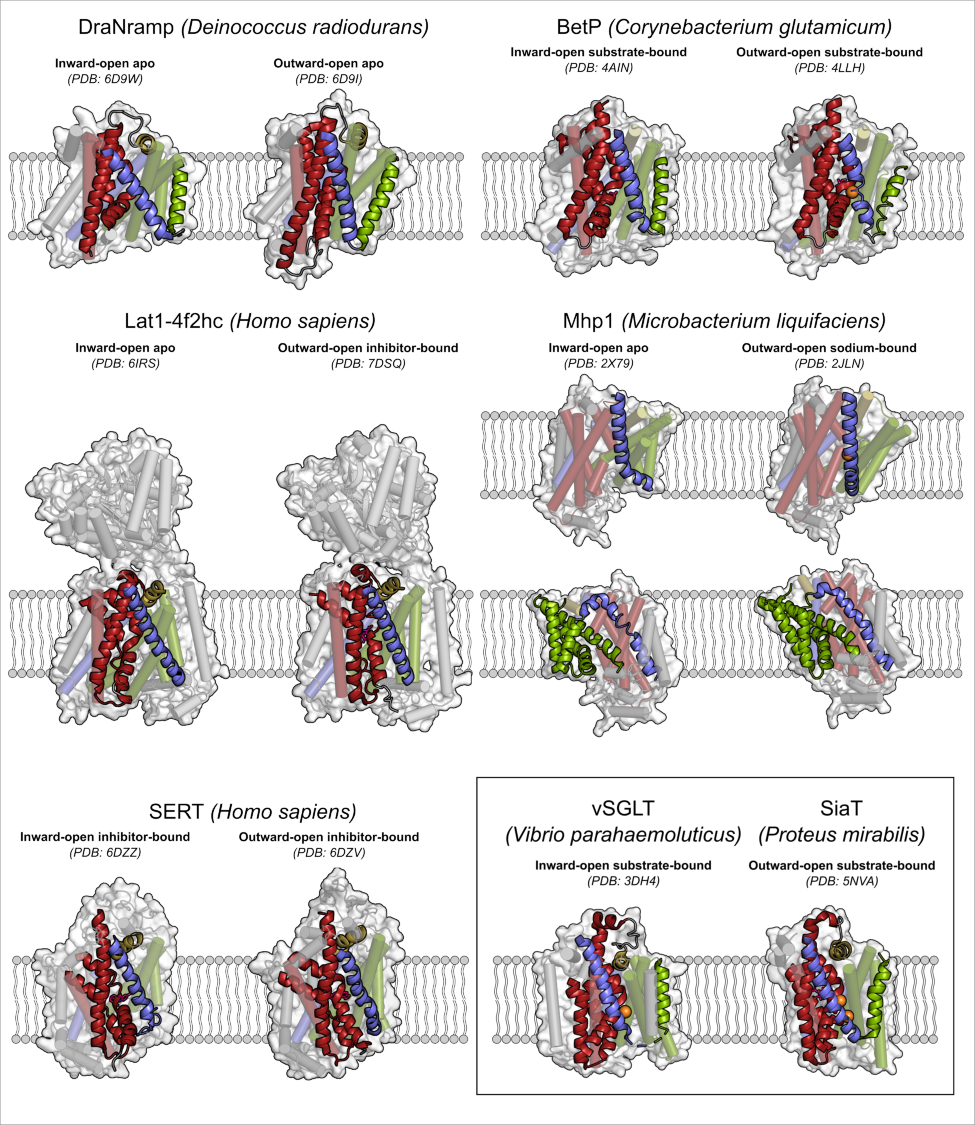
\includegraphics[width=6.5in]{Figures/leutintro_aa.pdf}
 \caption[Variations in structural dynamics within the LeuT-fold.]{Variations in structural dynamics within the LeuT-fold. Conformational dynamics of LeuT-fold transporters show striking differences in how alternating access is carried out. Dynamic and static helices are depicted as ribbons and cylinders, respectively. Bottom left: No individual \gls{sss} has been characterized in both \gls{of} and \gls{if} conformations.}
\label{fig:leutintro_aa}
\end{figure}

\begin{figure}[h!]
\centering
\includegraphics[width=6.5in]{Figures/leutintro_rmsf.pdf}
 \caption[Residue-level movements during IF-to-OF isomerization in various LeuT-fold proteins.]{Residue-level movements during \gls{if}-to-\gls{of} isomerization in various LeuT-fold proteins. Unresolved residues omitted from the plot. All structures were aligned using TM-Align \citep*{Xu2010, Zhang2005}.}
\label{fig:leutintro_rmsf}
\end{figure}

\subsection{Movement of gating helix TMH5}\label{sec:leutintro_tm5}

Along with the intracellular loop preceding it, \gls{tmh}5 ranks among the most consistently mobile and dynamic regions in the transporters studied so far \citep*{Stolzenberg2017}.  In \gls{of} conformations, \gls{tmh}5 nestles against the bundle domain helices \gls{tmh}1a and \gls{tmh}6b, forming the highly ordered intracellular "thick gate". In the IF state, by contrast, opening of the intracellular vestibule is driven by rearrangements that vary across families and even individual proteins within families. The contribution of \gls{tmh}5 to alternating access has been most extensively studied in \gls{nss}s \citep*{Stolzenberg2017}. A $\mathrm{G_{X}NP}$ sequence, strictly conserved within the family and partially conserved throughout the fold, putatively mediates both bending and unfolding motions instrumental to the initiation of substrate release (Figure \ref{fig:leutintro_tm5tm10}). Mutagenesis of glycine or proline severely abrogates transport \citep*{Malinauskaite2014}, highlighting the importance of the dynamic processes facilitated by this motif. First observed in a substrate-bound \gls{if}-occluded conformation of MhsT \citep*{Malinauskaite2014}, partial unwinding of \gls{tmh}5 has been corroborated in several \gls{nss}s by \gls{hdxms} studies under conditions promoting the \gls{if} conformation of each protein \citep*{Adhikary2017, Merkle2018, Moeller2019, Nielsen2019}. However, although \gls{if}-open structures of LeuT and \gls{sert} show this helix protruding out from the rest of the transporter \citep*{Coleman2016, Gotfryd2020, Krishnamurthy2012}, orthogonal measurements in LeuT both suggest that under \gls{if}-promoting conditions it adopts conformations where the intracellular cavity is occluded, rather than open \citep*{Kazmier2014, Shi2008, Zhao2011, Zhao2010}. As is elaborated below in Section \ref{sec:leutintro_nss_dynamics} below, however, these results are qualified by the frequent use of leucine, which has a low transport rate and nanomolar binding affinity \citep*{Singh2008}. Subsequent solution-state experiments bound to different amino acids found that quenching of fluorescent probes attached to the intracellular half of \gls{tmh}5 inversely correlated with transport rate \citep*{Billesbølle2015}, suggesting that this \gls{if}-occluded conformation may be less stable, relative to \gls{if}-open, when transporting substrates with higher turnover rates such as alanine. Nevertheless, in conjunction with other findings discussed below in Section \ref{sec:leutintro_nss_dynamics}, this points to a mechanism in which \gls{tmh}5 preferentially adopts the partially unwound occluded conformation when bound to its substrate but transiently bends to release substrates.

It is notable that \gls{tmh}5 adopts a similar, but not identical, conformation in \gls{if}-open Mhp1, which shares this $\mathrm{G_{X}NP}$ sequence \citep*{Shimamura2010}. Despite this agreement, \gls{epr} measurements revealed a degree of disorder in \gls{tmh}5 altogether absent from similar measurements carried out on LeuT in the presence of leucine \citep*{Kazmier2014a}. Interestingly, ApcT also shares a LeuT-like bend despite lacking a proline in \gls{tmh}5 at the equivalent position \citep*{Shaffer2009}. Since its structure has only been determined in a single conformation, and since its homologs such as GadC and BasC maintain a straight conformation of this helix \citep*{Jungnickel2018, Ma2012}, the extent to which the aforementioned \gls{nss} movements occur in ApcT and its homologs is unclear \citep*{Shi2010}. Finally, although \gls{tmh}5 is also involved in opening the intracellular cavity in DraNramp \citep*{Bozzi2019}, which also lacks the conserved mid-helical proline, it undergoes a rigid-body up-and-out translation rather than bending and unfolding. Many other \gls{if} structures, such as those observed in vSGLT and GkApcT, lack a fully resolved stretch of residues corresponding to \gls{il} 2, located between \gls{tmh}s 4 and 5, indicating a high degree of heterogeneity in the crystal lattice or \gls{cryoem} grid \citep*{Jungnickel2018, Watanabe2010}. Ultimately, the conformational variation observed across the fold in this loop and helix, combined with solution-state data indicative of local disorder, suggests that the protruded conformation observed in some proteins, though perhaps physiologically relevant and likely fundamental to the transport cycle, may not represent a well-defined low-energy state.

\begin{figure}[h]
\centering
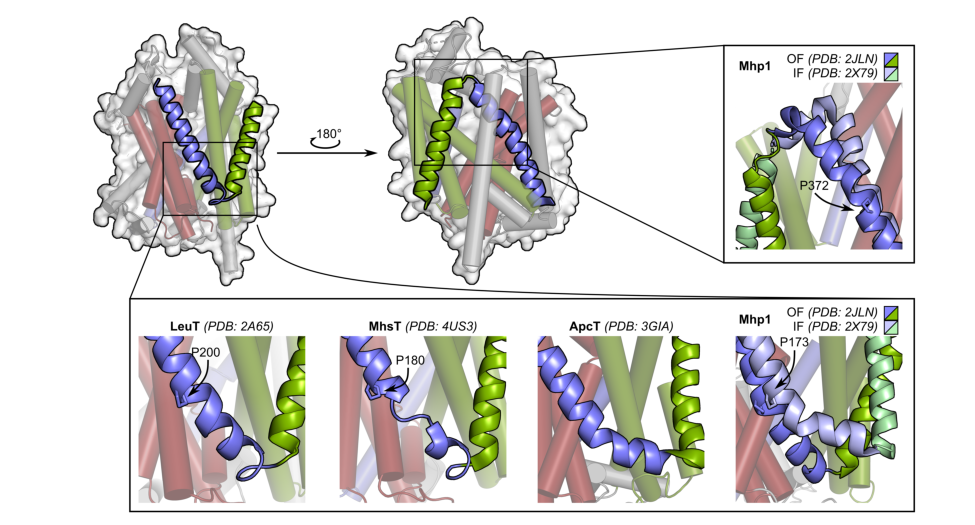
\includegraphics[width=6.5in]{Figures/leutintro_tm5tm10_hoz.pdf}
 \caption[Pivoting of TMH5 and TMH10 is observed in a subset of LeuT-fold transporters.]{Pivoting of \gls{tmh}5 and \gls{tmh}10 is observed in a subset of LeuT-fold transporters. Top left: LeuT with \gls{tmh}4/5 and TM9/10 highlighted. Bottom: Movements of \gls{tmh}5 observed in \gls{nss}s, ApcT, and DraNramp in the IF state. Conserved proline residues are highlighted in LeuT, MhsT and Mhp1. Top right: Movement of \gls{tmh}0 in Mhp1.}
\label{fig:leutintro_tm5tm10}
\end{figure}

\subsection{Movement in gating helix TMH10}

Movement in \gls{tmh}10, despite its pseudosymmetry to \gls{tmh}5, is less frequently observed (Figure \ref{fig:leutintro_tm5tm10}.B). In \gls{nss}s, for example, no evidence has been collected that show involvement in either ligand-dependent conformational dynamics, or partial unwinding \citep*{Kazmier2014a, Merkle2018, Moeller2019, Nielsen2019}. Mhp1 shows some partial symmetry of \gls{tmh}10 to \gls{tmh}5 in both sequence and structure, with comparable increases in conformational heterogeneity detected by \gls{epr} under \gls{of}-stabilizing experimental conditions (Figure \ref{fig:leutintro_tm5tm10}) \citep*{Kazmier2014, Shimamura2010, Weyand2008}. However, the movement inferred from crystal structures is less dramatic than that of \gls{tmh}5. In both BetP and DraNramp, differences between their \gls{of}-closed and open conformations in this region, though less drastic than in Mhp1, are nonetheless unmistakable; indeed, the corresponding proline in \gls{tmh}10 facilitating this bend is strictly conserved in the \gls{bcct} family and partially conserved among \gls{nramp}s \citep*{Bozzi2021, Schulze2010}. Although the \gls{apc} transporter AdiC both shares this specific residue and shows evidence of this structural movement, its structural similarity to the eukaryotic homolog Lat1, which instead has a cysteine at the equivalent position, indicates that placement of the proline halfway across \gls{tmh}10 may be coincidental \citep*{Fang2009, Yan2021}.

\subsection{Helical pivoting in the bundle domain}\label{sec:leutintro_bundle}

LeuT's twofold pseudosymmetry initially appeared to imply that a rigid-body rotation of the bundle domain relative to the rest of the structure mediates alternating access \citep*{Forrest2008}. This proposal, although elegant, failed to predict subsequent structural evidence in two key respects. First, the contribution of this domain to alternating access, although prominent in some proteins, is far from universal. Movement in ancillary helices and loop regions has been observed in every protein studied thus far. Second, the bundle domain virtually never moves as a rigid body. The exception, Mhp1, locks the bundle domain into place and instead pivots the hash domain and gating helices around this scaffold \citep*{Weyand2008} (see Section \ref{sec:leutintro_hash} below).

Movements in \gls{tmh}1a embody the variable intradomain dynamics observed in these helices. Its apparent dissociation from the rest of the intracellular vestibule, observed in X-ray and \gls{cryoem} structures of \gls{nss}s and \gls{nramp}s \citep*{Bozzi2019, Coleman2019, Ehrnstorfer2014, Krishnamurthy2012}, has been verified in solution (both families, it should be noted, lack N-terminal helices and oligomeric interfaces capable of restricting the dynamics of \gls{tmh}1a; see Figure \ref{fig:leutintro_rmsf}). Particular controversy surrounds the relevance of the signature 45° pivot observed in LeuT, which has been attributed to both the use of short-chain detergents commonly used in membrane protein crystallography \citep*{Moeller2020, Sohail2016}, as well as alanine mutagenesis of a conserved tyrosine residue essential for function \citep*{Krishnamurthy2012, Loland2002}. Molecular dynamics simulations of LeuT's \gls{if}-open crystal structure in a lipid bilayer later revealed the steep energetic cost of this movement into a more physiological membrane environment \citep*{Sohail2016}. Although this brought attention to the contribution of the membrane mimetic (along with a high-affinity antibody) in stabilizing such an extreme conformer, these findings, alongside experimental measurements obtained using both \gls{lret} \citep*{Sohail2016} and \gls{hdxms} \citep*{Adhikary2017} in lipid environments, nonetheless corroborated the more general hypothesis that \gls{tmh}1a becomes conformationally disordered in the \gls{if}-open state. Nevertheless, as these experiments were executed on similar tyrosine-to-alanine mutants, they do not address the extent to which this \gls{if}-open conformation is sampled by the wildtype protein in solution. For example, \gls{epr} measurements on equivalent tyrosine-to-alanine mutants recorded a comparable degree of disorder in \gls{tmh}1a; by contrast, no such dynamics were observed in variants without this mutation \citep*{Kazmier2014a, Merkle2018}. Follow-up experiments in \gls{sert} would paint a similar picture, with ibogaine, a ligand used to stabilize the \gls{if}-open structure during \gls{cryoem} studies, taking the role of this tyrosine-to-alanine mutation in LeuT \citep*{Coleman2019, Moeller2019}. Overall, the data suggest that the \gls{if}-open conformations of \gls{nss}s, and perhaps other proteins with similar conformational dynamics, transiently sample disordered \gls{tmh}1a states as part of their function, dovetailing with the conclusions on \gls{tmh}5 discussed above.

A similar pattern of increased disorder under \gls{if}-open-promoting conditions has also been observed in the intracellular side of \gls{tmh}7. In addition to the movements observed crystallographically, \gls{tmh}7 in LeuT appears to partially unfold under \gls{if}-favoring experimental conditions \citep*{Merkle2018}. For example, the eight N-terminal residues of this helix were not assigned to electron density in \gls{if}-open apo DraNramp \citep*{Bozzi2019}. The most pronounced motion of \gls{tmh}7 is likely found in Lat1, which swings over \SI{10}{\angstrom} to close its intracellular cavity \citep*{Yan2021}. As is discussed below, such a motion was suggested by, but not directly observed in, its bacterial homologs in the \gls{apc} family \citep*{Errasti-Murugarren2019, Ma2012}. Interestingly, no comparable movements are observed on the extracellular side of \gls{tmh}7. Unfortunately, the absence of data reporting the dynamics of transporters in the \gls{apc} family prevents any conclusions regarding increases in disorder in this helix from being established.

\gls{tmh}1b and \gls{tmh}6a, located on the extracellular sides of the protein, consistently undergo smaller scale but nonetheless significant dynamics essential to opening of the extracellular vestibule \citep*{Singh2008}. These helices appear to open the extracellular vestibule by moving in concert with the conserved helix \gls{el} 4, located between \gls{tmh}7 and \gls{tmh}8, in \gls{nss}s, \gls{apc} transporters, and \gls{nramp}s. While the observed movements of \gls{el}4 appear minor when compared to \gls{tmh}1a on the intracellular side, \gls{epr} spectroscopy data on LeuT indicate that crystal structures may understate the true extent to which these helices move \citep*{Kazmier2014}. Interestingly, on the intracellular side, no equivalent coupling between \gls{tmh}1a, \gls{tmh}6b, and \gls{il}1 has been detected to our knowledge. Indeed, unlike \gls{el}4, \gls{il}1 appears to be firmly stapled to the hash domain.

\subsection{The hash domain generally acts as a rigid body}\label{sec:leutintro_hash}

Relative to movements outlined above, independent helical movement within the hash domain are relatively rare. Mhp1 stands out in rocking this domain, alongside bending in \gls{tmh}5 and \gls{tmh}10, to fully mediate alternating access \citep*{Kazmier2014a, Shimamura2010, Weyand2008}. Similar movements were recorded in vSGLT using \gls{epr} \citep*{Paz2018}, although these coincided with additional movement distributed throughout the rest of the structure. As a point of contrast, other proteins limit their movements to bending of \gls{tmh}4 on the intracellular side and \gls{tmh}9 on the extracellular side to complement aforementioned movements of \gls{tmh}5 and \gls{tmh}10, respectively. The contribution of ancillary helices, which are frequently found adjacent to the hash domain, in explaining this phenomenon is unclear. In an interesting twist, a preprint publication describing the \gls{if}-to-\gls{of} transition in KCC1 proposes that alternating access is purely mediated by movement of \gls{tmh}3 and \gls{tmh}8, while \gls{tmh}4 and \gls{tmh}9 remain fixed \citep*{Liu2019, Zhao2020}.

\subsection{Conformational stabilization complicates the interpretation of these structures}

Importantly, many of these transporters, with Mhp1 and BetP being noteworthy exceptions, could only be coaxed into specific conformations using mutations, antibodies, or high-affinity transport inhibitors detrimental to function (see Tables \ref{tab:leutintro_proteins1} and \ref{tab:leutintro_proteins2}). In addition to the controversial use of a transport-abolishing tyrosine-to-alanine mutation in LeuT discussed above (Section \ref{sec:leutintro_bundle}) \citep*{Krishnamurthy2012}, stabilization of its \gls{if}-open state was also achieved by mutating a conserved tryptophan similarly found to be essential for function \citep*{Gotfryd2020}. Crystallographic capture of DraNramp in \gls{of} and \gls{if} conformations required glycine-to-arginine and glycine-to-tryptophan mutations near the unwound regions of \gls{tmh}1a and \gls{tmh}6a, respectively, that prevented isomerization by obstructing closure of the appropriate vestibule \citep*{Bozzi2016, Bozzi2019}. In human \gls{nramp}s, the equivalent missense mutation in \gls{tmh}1a is correlated with severely reduced iron uptake \emph{in vivo} \citep*{Barrios2012}, highlighting the extent to which transport function is impaired. Similarly, crystallization of \gls{if}-open vSGLT resulted from a lysine-to-alanine mutation that prevented ligand binding and showed no transport activity \citep*{Watanabe2010}. Capture of the OF-occluded conformation of AdiC, achieved using an aspartate-to-alanine mutation, may have played a role in stabilizing a ligand pose distinct from those observed in subsequent ligand-bound crystal structures of the wildtype protein \citep*{Gao2009}. Equivalent studies of the eukaryotic transporters \gls{sert} \citep*{Coleman2019}, Lat1 \citep*{Yan2021}, and KCC1 \citep*{Zhao2020} have employed a broad panel of potent inhibitors that preferentially bind to specific conformations. Whereas apo \gls{sert} readily crystallized in an \gls{of} conformation, capture of its \gls{if} conformation required the small molecule ibogaine \citep*{Coleman2019}. Similarly, both Lat1 and KCC1 were structurally characterized in \gls{if} conformations in the absence of ligands \citep*{Lee2019, Liu2019, Xie2020, Yan2020a} but could only be described in \gls{of} conformations using inhibitors \citep*{Yan2021, Zhao2020}. In each of these cases, the introduction of small molecules and/or inactivating mutations arrested transport by stabilizing conformers off-path with respect to the protein's functional cycle.

Nevertheless, assuming the physiological relevance of these structures, their comparison naturally prompts speculation regarding the evolutionary and/or functional basis for the variation in alternating access mechanisms. One proposal, made by the authors that determined the \gls{of} structure of KCC1, is the size of the ligand; only small-scale movements, limited to \gls{tmh}3 and \gls{tmh}8, are necessary for symport of the relatively small ions potassium and chloride \citep*{Zhao2020}. This hypothesis implies that larger substrates require larger movements and is supported by the observation that outward-locked DraNramp can transport protons, but not metals \citep*{Bozzi2019}. However, the small size of metals nonetheless raises questions about why DraNramp's \gls{of}-to-\gls{if} transition consists of such large-amplitude movements. Similarly, the relatively minor conformational changes observed in the transport cycle of BetP \citep*{Perez2012}, the substrates of which are comparable in size to amino acids, have been justified by function-specific adaptations. Ultimately, the insufficient data prevent any conclusions from being established in this respect.

\section{Connecting the dots: from structures to landscapes}

Proteins rarely navigate the conformational space accessible to them in the stepwise fashion suggested by depictions such as the one shown in Figure \ref{fig:leutintro_nss}. Mechanistic models of transport must necessarily, therefore, also map the conditions under which specific conformations occur. Secondary active transporters lack a molecular motor such as an ATPase and must therefore rely on the energy input provided by ions and ligands to undergo forward transport \citep*{Boudker2010}. The central question concerns how transporters harness this energy to undergo reconfigurations that ultimately result in productive transport. Unfortunately, the outstanding structural record of the LeuT-fold overrepresents static states amenable to structural characterization \citep*{Mullen2016, Tsai2010}. As a result, although the resulting structures enrich mechanistic models of transport, such as the glide-symmetry symport mechanisms proposed over two decades ago for \gls{nss}s \citep*{Rudnick2006} and \gls{ccc}s \citep*{Russell2000}, they are ill-equipped to directly test them. An example that will not be discussed further is the possible existence of an allosteric binding site in LeuT and other prokaryotic \gls{nss}s, which remains controversial despite over a decade of structural and experimental research \citep*{Fitzgerald2019, LeVine2019, Merkle2018, Piscitelli2010, Quick2009, Quick2012, Shi2010, Tavoulari2011}.

\subsection{Characterizing dynamics in the NSSs}\label{sec:leutintro_nss_dynamics}

The energy landscapes of \gls{nss}s are far better characterized than thoose of LeuT-fold proteins in other families and point to a striking degree of conservation. Measurements carried out in solution consistently demonstrate that sodium stabilizes OF conformations, ligands stabilize occluded conformations, and absence of either promotes flexible interconversion between \gls{if}-open and \gls{of}-open \citep*{Kazmier2014, Merkle2018, Terry2018, Zhang2018, Zhang2021}. These data provide additional context for these structures by reporting on how ligand-binding events bias the conformational ensemble, which can hint at the drivers of the transport cycle. At the same time, the data can reveal steps unanticipated by canonical symport and/or antiport mechanisms. For example, recent data suggesting that potassium stabilizes \gls{if}-open LeuT hint at a step in which intracellular potassium ions indirectly participate in the transport cycle by competing with sodium and accelerating their release from the central binding site \citep*{Billesbølle2016, Merkle2018} (facilitation of substrate release by allosterically bound ions has since been reported in KCC1 \citep*{Liu2019} and KCC2 \citep*{Zhang2021a} and suggested for KCC4 \citep*{Reid2020}).

These studies further highlight how homologs might diverge due to functional specialization. Despite their structural similarity, LeuT, \gls{sert} and \gls{dat} were observed to have slight variations in their conformational dynamics. Whereas LeuT adopts an \gls{if}-occluded conformation when bound to leucine \citep*{Kazmier2014a, Merkle2018}, \gls{sert} fluctuates between \gls{if}-occluded and \gls{if}-open \citep*{Moeller2019}. More intriguingly, the helical unwinding in \gls{il}2 and \gls{tmh}5 initially proposed by the \gls{if}-occluded structure of MhsT \citep*{Malinauskaite2014}, although plausible in LeuT and \gls{sert}, was altogether inconsistent with data collected in \gls{dat} suggesting a lack of cooperative movement in this region \citep*{Nielsen2019}. Comparable dynamics were instead observed in \gls{il}4, a nearby region that was previously found to be critical to \gls{if}-opening in other eukaryotic \gls{nss}s but static in LeuT \citep*{Hansra2004, Kazmier2014a} (lack of coverage in \gls{hdxms} studies of \gls{sert} prevented this region from being studied \citep*{Moeller2019}). However, the presence of lipids and cholesterol in \gls{dat} samples presents a confounding factor when attempting to directly compare these results to those collected in \gls{sert}, which was studied in detergent micelles. This suspicion is supported by previous studies that reported modulation of conformational dynamics in both eukaryotic \gls{nss}s and other secondary active transporters by detergent and lipids \citep*{Coleman2019, Damian2021, Jagessar2020, Martens2016, Moeller2019, Penmatsa2013, Zakrzewska2019}.

\begin{figure}[H]
\centering
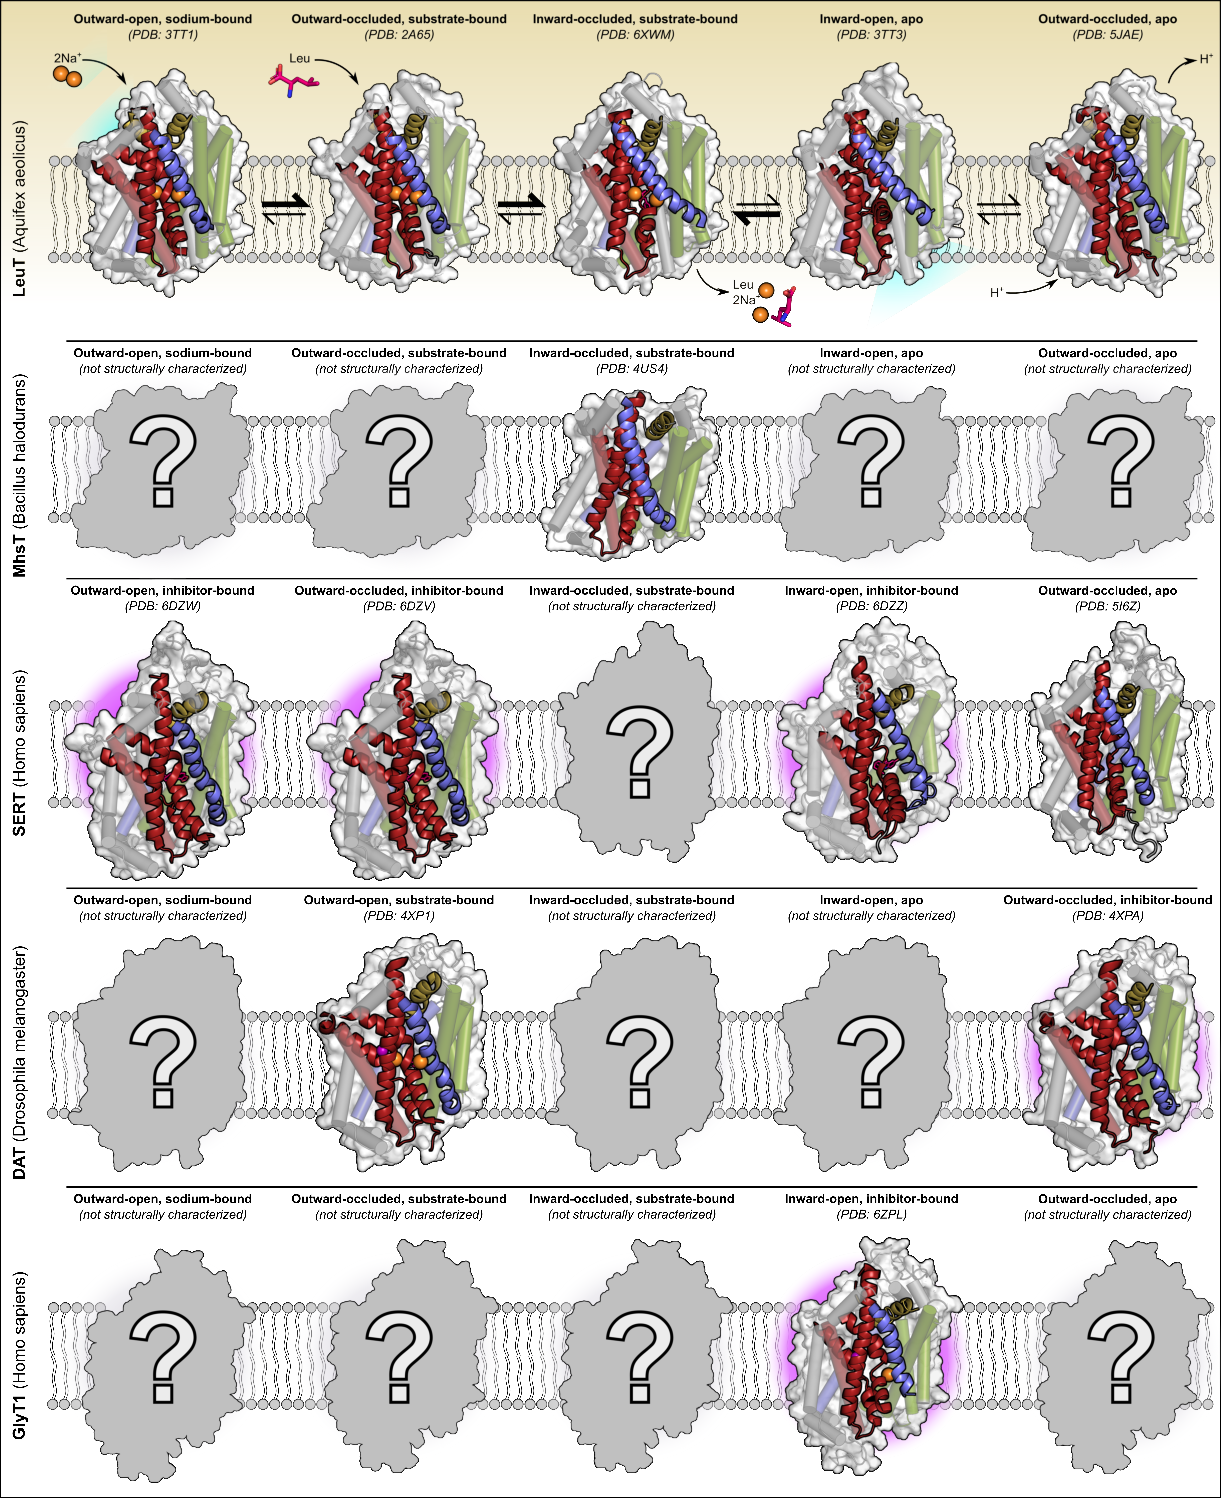
\includegraphics[width=6.5in]{Figures/leutintro_nss.pdf}
 \caption[Conformational dynamics of neurotransmitter-sodium symporters inferred from crystal structures.]{Conformational dynamics of neurotransmitter-sodium symporters inferred from crystal structures. Top: LeuT couples the import of small aliphatic amino acids, such as leucine, to the inward and outward electrochemical gradients of sodium and protons, respectively. Bottom: Incomplete transport cycles of other \gls{nss}s. Inhibitor-bound states are highlighted in purple.}
\label{fig:leutintro_nss}
\end{figure}

Single-molecule visualization of conformational changes using \gls{fret} has added a layer of detail entirely missed by these ensemble-level measurements \citep*{Juette2014, Schuler2013}. A recent study employing this technique showed how LeuT appears to undergo uncoupled movement on the intracellular and extracellular sides of the membrane in the absence of substrate, including sampling a channel-like conformation simultaneously open to both sides \citep*{Terry2018}. Although canonical symport mechanisms of alternating access forbid this arrangement \citep*{Forrest2009}, LeuT appears to avoid uncoupled sodium flux by sealing the intracellular cavity in response to sodium binding. Additionally, this study corroborated previous experimental and computational studies on LeuT suggesting that substrate dissociation, and specifically ligand-dependent sodium dissociation from the Na2 site (see Section \ref{sec:ligands} above) \citep*{Billesbølle2015, Razavi2018}, is the rate-limiting step in transport. However, as mentioned above, this phenomenon may be unique to LeuT. A subsequent study on wildtype MhsT, in which soluble amino acid-binding proteins labeled with pairs of complementary fluorescent probes were cleverly introduced to the interior of MhsT-containing proteoliposomes, determined that the substrate-free \gls{if}-to-\gls{of} transition was instead rate-limiting \citep*{Fitzgerald2019}. Electrophysiology studies in human \gls{nss}s led to similar conclusions \citep*{Bhat2021}, suggesting that these discrepancies may be attributable to lower rates of transport and/or higher ligand-binding affinity observed in the thermophilic protein LeuT relative to transporters adapted to function at lower temperatures. 

\subsection{Differential dynamics in the SSS family}

The differences in conformational dynamics among \gls{nss}s, although not trivial, are dwarfed by those distinguishing them from \gls{sss}s such as the eukaryotic sodium/glucose symporter SGLT1, the prokaryotic sodium/galactose symporter vSGLT, and the prokaryotic sodium/proline symporter PutP. While not as well studied, these proteins traverse an energy landscape that is distinct from those of \gls{nss}s and indicative of the challenges inherent to the interpretation of solution-state dynamics data. \Gls{epr} measurements of vSGLT \citep*{Paz2018} and PutP \citep*{Raba2014} as well as fluorescent labeling and cysteine accessibility measurements in SGLT1 \citep*{Loo1998, Loo2006, SalaRabanal2012} suggest that ligand-dependent conformational dynamics were effectively inverted relative to \gls{nss}s, with apo and/or sodium-rich conditions favoring \gls{if} conformations and substrate binding stabilizing the \gls{of} conformation. As with \gls{nss}s discussed above, key differences between vSGLT and PutP were observed: no conformational response to sodium binding was detected in the former \citep*{Paz2018}, whereas sodium binding to the latter led to closing of \gls{el}4 and increased labeling of residues lining the intracellular vestibule \citep*{Jeschke2004a, Raba2014, Wegener2000}. Importantly, similar sodium-invariant conformational dynamics were independently reported in the unrelated bacterial transporter Mhp1 using both \gls{epr} and cysteine accessibility measurements \citep*{Kazmier2014, Calabrese2017, Weyand2011}, and sodium-driven stabilization of an \gls{if} state was also suggested by \gls{epr} data in BetP \citep*{Leone2019}.

Data from \gls{epr} studies on vSGLT prompted the conclusion that the sodium gradient is a critical driver of transport \citep*{Paz2018}. Consistent with this hypothesis, accessibility measurements and fluorescent labeling data collected in human SGLT1 in cells that actively maintain a sodium gradient showed a conformational landscape nearly identical to \gls{nss}s: unrestricted isomerization between \gls{of} and \gls{if} in the apo state \citep*{SalaRabanal2012} and stabilization of the \gls{of} conformation in the presence of sodium and absence of glucose \citep*{Loo1998, Meinild2002}. Critically, the \gls{of}-promoting effect of sodium diminished when the electrochemical gradient was decreased \citep*{Loo1998}. However, while these data support the hypothesis that the gradient may play a similar role in prokaryotic \gls{sss}s, a critical difference with unknown significance is SGLT1’s 2:1 sodium-to-glucose stoichiometry, which contrasts with the 1:1 stoichiometry of the prokaryotic model systems discussed above. 

\subsection{Energy landscapes in antiporters}\label{sec:leutintro_antiporters}

Missing from our knowledge of transporters with this fold is a detailed accounting of conformational dynamics data in antiporters. Despite their ubiquity in all domains of life and their extensive structural study by crystallography and \gls{cryoem} (Figure \ref{fig:leutintro_apc}), their energy landscapes remain virtually uncharacterized. Whereas canonical symport mechanisms, such as those broadly defining \gls{nss}s and \gls{sss}s, contain a substrate-free isomerization step, canonical antiport mechanisms facilitate substrate exchange by forbidding this conformational change \citep*{Forrest2009}. Instead, the second half of the antiport cycle involves the translocation of a second substrate in the opposite direction. In non-LeuT-fold antiporters, import of one molecule is proposed to power the energetically unfavorable export of another. For example, mechanisms of alternating access in unrelated transporters that expel toxic drugs frequently involve the cation-dependent stabilization of an \gls{if} conformation \citep*{Eisinger2017, Jagessar2020, Masureel2014}. The relevance of these findings to understanding LeuT-fold antiporters, however, is unclear, since many of them are not coupled to electrochemical ion gradients and instead function as substrate exchangers facilitating downhill translocation in opposite directions \citep*{Fang2009, Ma2012, Schulze2010, Tang2010}.

\begin{figure}[H]
\centering
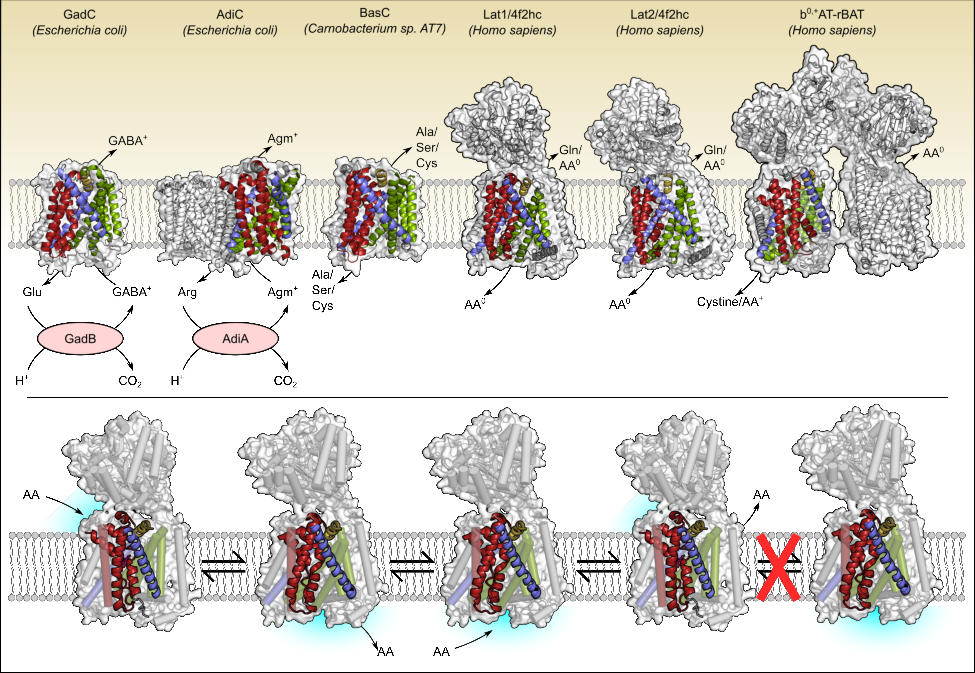
\includegraphics[width=6.5in]{Figures/leutintro_apc.pdf}
 \caption[Structures and transport cycles of amino acid exchangers in the APC family.]{Structures and transport cycles of amino acid exchangers in the APC family. Top: The pH-activated precursor-product exchangers GadC and AdiC are co-transcribed with decarboxylases GadB and AdiA, respectively. Bottom: Canonical mechanisms of antiport forbid substrate-free conformational isomerization.}
\label{fig:leutintro_apc}
\end{figure}

A range of pH-dependent amino acid/polyamine antiporters in the \gls{apc} family, sometimes called "virtual proton pumps", import and export the precursors and products, respectively, of proton-consuming amino acid decarboxylases with which they are cotranscribed (Figure \ref{fig:leutintro_apc}) \citep*{Fang2009, Foster2004, Kanjee2013, Krammer2019, Ma2012}. Activation of these decarboxylases under extreme acidic conditions drains the intracellular concentration of the appropriate amino acids and raises that of the cognate polyamines, thus ensuring that both halves of the antiport cycle are energetically favorable. In fact, the two most well-characterized transporters, AdiC and GadC, are capable of forward and reverse transport of both substrates under equilibrium conditions \citep*{Ma2012, Ma2013, Tsai2013, Tsai2013a}. In contrast, they are inactive when their intracellular sides, but not extracellular sides, are exposed to protons, or in the presence of a negative-inside electric potential \citep*{Tsai2013, Tsai2013a}. One hypothesis proposed from \gls{md} simulations of AdiC posits that protonation of a conserved glutamate leads to the rate-limiting substrate dissociation from the central binding site \citep*{Zomot2011}, similar to the proposed role of potassium-induced substrate release on the intracellular side of LeuT (see section \ref{sec:leutintro_nss_dynamics}).

Homologs with broader substrate specificities such as BasC and Lat1 exchange amino acids in accordance with cellular needs while maintaining high intracellular amino acid concentrations \citep*{Errasti-Murugarren2019, Lee2019, Yan2019}. A critical adaptation in these proteins is their asymmetric binding affinity, with apparent Km values in the micromolar and millimolar range during out-to-in and in-to-out transport, respectively \citep*{Bartoccioni2019}. This is hypothesized to address the disparity between amino acid concentrations on the intracellular and extracellular side, which differ by several orders of magnitude. A secondary form of asymmetry in amino acid exchangers of the APC family is the selective import and export of charged substrates; $\mathrm{b^{(0,+)}AT1}$ selectively imports and exports cationic and neutrally charged amino acids, respectively, although neither the structures nor subsequent studies have shed light on the structural basis of this observation \citep*{Wu2020, Yan2020a}.

Unfortunately, the recent explosion of structures in the \gls{apc} transporter family has not been accompanied by studies into these proteins' energy landscapes. To our knowledge, the only study of dynamics in antiporters in the \gls{apc} family has been in the bacterial serine/threonine antiporter SteT \citep*{Reig2007} using single-molecule dynamic force spectroscopy, which reports on a protein's kinetic barriers \citep*{Bippes2009}. This study found that conformational flexibility in SteT increased under substrate-bound conditions relative to apo, consistent with the substrate-dependent conformational movement predicted by a canonical model of antiport. However, the data do not report on the protein's thermodynamics, which leaves critical questions about the protein's energy landscape unanswered.

\section{Comparison to homologous proteins}\label{sec:leutintro_homologs}

Overall, the outstanding evidence suggests that proteins in the LeuT-fold share few, if any, signature motifs of alternating access. To answer the question posed in the Introduction, differences in the structures and conformational dynamics of transporters both within and across families suggest that functional specialization has contributed to a degree of evolutionary divergence that prevents our rich knowledge of \gls{nss}s in general and LeuT in particular from being directly applied to less well-known families such as \gls{kup}s or \gls{aaap}s. However, the data also suggest that transporters in the same family are more similar to each other, both in structure and dynamics, than to proteins in other families. Thus, the question is one of evolutionary conservation at the family-level.

\subsection{Structural similarity within families of transporters}

From the perspective of structural similarity, the outstanding data suggest that homologs within a protein family show a degree of structural conservation not shared by other proteins with this fold. During their transport cycles, individual proteins sample conformations that differ by \SI{3}{\angstrom} $\mathrm{C_{\upalpha}}$ \gls{rmsd} \citep*{Ponzoni2018}. Structures of homologous proteins within and across families, meanwhile, differ by around \SI{3}{\angstrom} and \SI{5}{\angstrom} $\mathrm{C_{\upalpha}}$ \gls{rmsd}, respectively. This divergence has complicated the development of unified mechanistic models of transport for any protein or family because structural variation between different proteins could either reflect differences in sequence and function, or represent distinct steps in the transport cycle. Indeed, minor structural differences are even observed when comparing the structures of the same protein across different species, such as CaiT from \emph{Proteus mirabilis} and \emph{Escherichia coli} \citep*{Schulze2010}, AdiC from \emph{Salmonella typhimurium} and \emph{E. coli} \citep*{Fang2009}, NKCC1 from \emph{Homo sapiens} \citep*{Yang2020, Zhang2021a} and \emph{Danio rerio} \citep*{Chew2019}, and KCC4 from \emph{H. sapiens} \citep*{Xie2020} and \emph{Mus musculus} \citep*{Reid2020}.

An instructive example that was discussed in Section \ref{sec:leutintro_tm5} above is the varying position of \gls{tmh}5 in \gls{nss}s. The ligand-bound \gls{if}-occluded structure of MhsT \citep*{Malinauskaite2014, Stolzenberg2017} was interpreted as evidence that unwinding of \gls{tmh}5 is a feature preceding substrate release in all \gls{nss}s. In contrast, the conformation of \gls{tmh}5 in \gls{if}-occluded LeuT, which was corroborated by \gls{fret}, was bent and not unwound, which provided comparatively greater access to the intracellular vestibule \citep*{Gotfryd2020, Terry2018}, while the conformation of \gls{tmh}5 in \gls{if}-occluded \gls{sert} was described as "halfway" between that of LeuT and MhsT \citep*{Coleman2019}. It remains unclear if these structures represent distinct steps in a shared transport cycle, or if they reflect more fundamental differences between proteins resulting from functional specialization, evolutionary divergence, and/or environment-specific adaptations.

\subsection{Structural similarity between prokaryotic and eukaryotic transporters}

Nevertheless, the striking degree of structural correlation observed between distantly related proteins, particularly between bacterial and eukaryotic proteins, has been a recurring theme throughout studies of proteins with this fold. The first eukaryotic LeuT-fold transporter to be structural determined, the dopamine transporter \gls{dat} from \emph{Drosophila melanogaster} \citep*{Penmatsa2013}, bore a remarkable resemblance to LeuT, obtained from a thermophilic archaeum found in hot springs. Similarly, the structure of the \gls{apc} transporter GadC in an \gls{if} conformation \citep*{Ma2012} aligns well with those determined for the eukaryotic transporters Lat1/4f2hc \citep*{Lee2019, Yan2021, Yan2019}, Lat2/4f2hc \citep*{Jeckelmann2020, Yan2020}, and $\mathrm{b^{(0,+)}AT1}$ \citep*{Wu2020, Yan2020a}. This observation is all the more intriguing given that GadC's structure putatively represents an auto-inhibited state with no mechanistic equivalent in the transport cycles of these eukaryotic proteins \citep*{Ma2012, Ma2013}. Equally fascinating is the correspondence between the \gls{of}-open inactive conformations of Lat1 \citep*{Yan2021} and AdiC \citep*{Ilgu2016}. Unfortunately, comparison of eukaryotic and bacterial homologs is only possible in the \gls{nss} and \gls{apc} families, as the structurally determined proteins comprising every other family of transporters are either exclusively prokaryotic or exclusively eukaryotic.

Regarding the energy landscapes of these proteins, a dearth of dynamics data prevents straightforward comparisons from being made. It is nonetheless remarkable that the structural dynamics of vSGLT are more similar to those of Mhp1, which has identical 1:1 sodium-to-substrate stoichiometry despite being unrelated at the sequence level, than those of its homolog SGLT1, which instead mirror those of \gls{nss}s sharing its 2:1 sodium-to-substrate stoichiometry \citep*{Kazmier2014, Loo1998, Paz2018}. At the same time, given the variation in dynamics data observed among NSSs \citep*{Adhikary2017, Kazmier2014a, Merkle2018, Moeller2019}, small divergences in how \gls{sss}s respond to their substrates at the structural level appear to be expected.

\subsection{Implications of structural similarity and divergence on modeling}\label{sec:leutintro_modeling}

In 2008, vSGLT became the second protein, after LeuT itself, to be observed with the LeuT-fold \citep*{Faham2008}. Publication of its crystal structure in an \gls{if} conformation was complemented by an \gls{of} model generated from the structure of LeuT that attempted to predict which helices are involved in alternating access. Though this comparison is, with the benefit of hindsight, somewhat inappropriate, modeling of alternate conformers has since been a staple of structural studies that has guided experimental design \citep*{Geier2013, Gotfryd2020, Paz2018, Napolitano2017, Ylikangas2014}, generated starting points in simulations \citep*{Bisignano2018, Kelashvilli2015, Razavi2018}, and contextualized experimental findings \citep*{Kazmier2014a, Paz2018, Terry2018}. The previous discussion emphasized the risk of assuming that conformations observed in one protein are relevant to others, modeling has been particularly effective at extracting mechanistic insights into eukaryotic proteins from bacterial model systems \citep*{Bisignano2018, Forrest2008, Forrest2007, Geier2013, Wang2013, Zomot2007}.

Shortly after structure determination of LeuT in 2005, modeling studies led to the identification of the chloride-binding site of eukaryotic \gls{nss}s \citep*{Forrest2007, Zomot2007}. Chloride ions are not native ligands of LeuT, which instead exchanges two extracellular sodium ions and an amino acid with an intracellular proton \citep*{Zhao2010}. Nevertheless, by identifying a negatively-charge side chain near the sodium binding site exclusive to chloride-independent \gls{nss}s \citep*{Beuming2006}, this chloride-transporting phenotype could be introduced by mutating native glutamate and aspartate near the sodium-binding site of LeuT and the bacterial \gls{nss} Tyt1, respectively \citep*{Zomot2007}. Likewise, chloride-independent transport could be introduced in the \gls{gaba} transporter GAT1 by replacing the serine in the same position with a glutamate. In parallel, the chloride-binding site in \gls{sert} was identified by aligning its sequence to LeuT, and the resulting homology model predicted the chloride-binding position in \gls{sert} with astonishing detail \citep*{Forrest2008}.

Several drug discovery studies of Lat1 employed homology models, generated from \gls{if}-occluded ApcT \citep*{Shaffer2009} and \gls{of}-open AdiC \citep*{Gao2009}, to guide rational design of inhibitors and ligands \citep*{Geier2013, Napolitano2017, Singh2018, Ylikangas2014}. Although small details in the substrate-binding sites of these models were subsequently found to be inconsistent with the \gls{cryoem} structures \citep*{Lee2019, Yan2021, Yan2019}, they nonetheless facilitated the identification of multiple novel inhibitors. One of these inhibitors was later used to trap Lat1 in an OF-open conformation for \gls{cryoem} studies \citep*{Yan2021}, and the resulting structures verified the "carboxylate-up" orientation initially predicted by the homology model that had been observed in other transporters (Figure \ref{fig:leutintro_ligands}).

Finally, structural models have been invaluable in guiding restraint selection using sparse experimental data. A model of \gls{of} vSGLT, generated from the homologous SiaT \citep*{Wahlgren2018}, was used to determine which measurements to pursue using \gls{epr} \citep*{Paz2018}. Importantly, the \gls{of} model provided a context for the relatively sparse distance data and highlighted the flexibility of \gls{tmh}10 that was unanticipated. Additionally, prior to the structural determination of NKCC1 by \gls{cryoem}, cross-linking experiments were guided by computational models generated from AdiC; the conformation and register of \gls{tmh}s 10-12 predicted by this model was subsequently validated by \gls{cryoem} \citep*{Monette2014, Yang2020}.

\section{Scope of this dissertation}

The objectives of this dissertation are twofold.

The first objective focuses on studying the structural dynamics of the glutamate/GABA antiporter GadC. At low pH, GadC serves as a model system for other LeuT-fold antiporters, particularly those in the APC sub-family, while at high pH it putatively adopts an inactive conformation. As was discussed in section \ref{sec:leutintro_antiporters}, these transporters are far less well studied than homologous sodium-coupled symporters, and the extent to which their mechanisms of alternating access are conserved is unclear. Symporters such as LeuT, Mhp1, PutP, vSGLT, and SERT have been shown to undergo ligand-dependent changes in their conformational equilibria; whether GadC or homologous exchangers found in eukaryotes do the same is unknown. These questions are explored in Chapter \ref{ch:gadc} using \gls{epr} spectroscopy and computational modeling.

As will be discussed in Chapter \ref{ch:intro_deer}, the experimental data collected in GadC can report on changes in the distribution of distances between two spin labels but are local in nature and must be complemented with computational modeling to obtain global, fold-level structural insights. Thus, the second objective of this dissertation focuses on developing novel computational methods to model the structures of these proteins using these data. The Markov Chain Monte Carlo approach used throughout this text separates the modeling process into two steps, sampling and scoring. As is discussed in subsequent chapters, existing sampling and scoring methods do not effectively leverage the experimental data, leading to unacceptable losses in modeling precision and unnecessary increases in computation time. Therefore, this dissertation describes and discusses advancements in both halves of the modeling process. However, more attention is paid to the development of scoring approaches; the novel sampling approach is discussed further in Appendix \ref{app:confchangemover}. These sampling and scoring methods are combined to attempt to model conformational changes in three homologs of GadC using experimental \gls{epr} data.

One thread discussed in chapters \ref{ch:rosettadeer} and \ref{ch:multilateration} of this dissertation, unrelated to these two objectives, explores the extent to which the analysis of \gls{deer} data and its use for computational modeling can be integrated. In general, the time-domain data are first interpreted as distance distributions, which are in turn used as modeling restraints (see Chapter \ref{ch:intro_deer} for details). While several recent reports have begun to couple interpretation of the time domain data with structural modeling, the benefits of this approach have not been studied. Chapters \ref{ch:rosettadeer} and \ref{ch:multilateration} explore these approaches in greater detail for two specific tasks, predicting the folds of protein structures using sparse \gls{deer} and determining the positions of nitroxide rotamers, respectively. The goal of these two chapters is to determine the extent to which these two steps can be coupled. As is discussed in Chapter \ref{ch:rosettadeer}, this has the potential to advance the integration of computation and spectroscopy in a manner analogous to the prediction of protein structures using unassigned \gls{nmr} chemical shifts or raw SAXS scattering profiles. An overview of methods to analyze and simulate \gls{deer} data is provided in the following chapter. %As we discuss in section \ref{sec:multilateration_main_intro}, this has the potential to avoid propagating artifacts introduced during data analysis, which may negatively affect the quality of structural models.

%The work presented here focuses on studying and modeling the structure of GadC, a glutamate/GABA antiporter that is only active at low pH. Critical unanswered questions surround the effect of substrate on the transport cycles of antiporters in general as well as GadC's pH-dependent activation mechanism in particular. Both questions are answered using \gls{epr} studies comparable to those carried out in LeuT, Mhp1, and vSGLT mentioned earlier. Importantly, while these measurements are executed in the absence of a pH gradient, they are performed on protein reconstituted into lipid nanodiscs that more faithfully recapitulate the protein's native environment. Nevertheless, due to the low information content of \gls{epr}, modeling is necessary to translate these pairwise distance measurements into mechanistic insights. Thus, considerable attention is paid to the development of methods capable of accurately modeling structural states using these data, which are briefly reviewed in Chapter \ref{ch:intro_deer}. Chapter \ref{ch:rosettadeer} and Appendices \ref{app:scoring} and \ref{app:rosettadeer_supp} cover the methods developed for modeling proteins using \gls{deer} data. Chapter \ref{ch:multilateration} and Appendices \ref{app:confchangemover} and \ref{app:multilateration_supp} use these data to model conformational changes in several benchmark cases. Finally, Chapters \ref{ch:gadc} and \ref{app:gadc_supp} unite these methodological advancements and model the structure of GadC using experimental data collected at low and neutral pH. Chapter \ref{ch:conclusions} discusses the challenges that methods development must address to improve the precision of protein structural models, as well as how these integrative approaches might be applied in light of recent advancements in the field of structural biology.

